\documentclass[12pt]{standalone}
\usepackage{tikz, amssymb} 
%\usetikzlibrary{calc, arrows.meta, decorations.pathreplacing}

\newcommand{\fourdots}{
  \fill (0,0) circle[radius=3.5pt];
  \fill (0,1) circle[radius=3.5pt];
  \fill (1,0) circle[radius=3.5pt];
  \fill (1,1) circle[radius=3.5pt];
}

\begin{document}

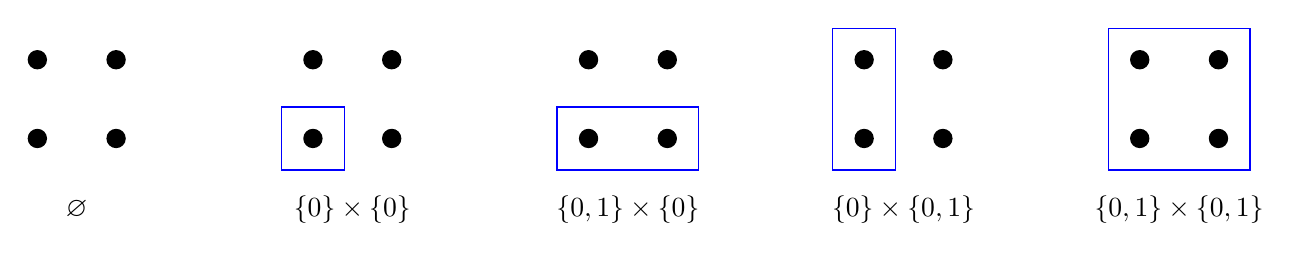
\begin{tikzpicture}[scale=1]
  \fourdots
  \node at (0.5, -0.9) { $\varnothing$};

  \begin{scope}[shift={(3.5,0)}]
    \draw[blue] (-0.4, -0.4) rectangle (0.4, 0.4);
    \fourdots
    \node at (0.5, -0.9) { $\{0\} \times \{0\}$};
  \end{scope}
  
  \begin{scope}[shift={(7,0)}]
    \draw[blue] (-0.4, -0.4) rectangle (1.4, 0.4);
    \fourdots
    \node at (0.5, -0.9) { $\{0,1\} \times \{0\}$};
  \end{scope}
  
  \begin{scope}[shift={(10.5,0)}]
    \draw[blue] (-0.4, -0.4) rectangle (0.4, 1.4);
    \fourdots
    \node at (0.5, -0.9) { $\{0\} \times \{0,1\}$};
  \end{scope}
  
  \begin{scope}[shift={(14,0)}]
    \draw[blue] (-0.4, -0.4) rectangle (1.4, 1.4);
    \fourdots
    \node at (0.5, -0.9) { $\{0,1\} \times \{0,1\}$};
  \end{scope}
\end{tikzpicture}

\end{document}
